% IEEE Transactions on Human-Machine Systems, special issue on Brain Discovery
% and Neurotechnology. Two-column IEEEtran is mandatory at submission: the editor
% uses it to judge length against the 10-page limit for a regular paper.
%
% Build:  make        (needs pdflatex + bibtex + IEEEtran.cls)
% or drop this folder into Overleaf, which ships IEEEtran.

\documentclass[journal]{IEEEtran}

\usepackage{graphicx}
\usepackage{amsmath}
\usepackage[T1]{fontenc}
\usepackage[utf8]{inputenc}
\usepackage{url}

\begin{document}

\title{Sensorimotor Rhythm or Aggregate Power? An Interpretability Audit of
EEGPT on Motor Imagery}

\author{Author Names%
\thanks{Affiliation placeholder. Corresponding author: e-mail placeholder.}}

\markboth{IEEE Transactions on Human-Machine Systems}%
{Author \MakeLowercase{\textit{et al.}}: Interpretability Audit of EEGPT on Motor Imagery}

\maketitle

\begin{abstract}
EEG foundation models match feature engineered baselines, yet recent audits
report they lean on the aperiodic $1/f$ background and its broadband power more
than on the specific oscillations that carry task meaning. We audit EEGPT, a
model absent from those audits that adds a spatio temporal representation
alignment objective to masked reconstruction, on PhysioNet motor imagery
(imagery versus rest, 35 subjects). A linear classifier on its frozen embeddings
decodes the task at ${\approx}71\%$ within subject, yet the embedding geometry is
dominated by aggregate, largely aperiodic power, correlating with a total-power
reference at Spearman $r \approx 0.24$--$0.32$, above any single band. The
evidence for rhythm specificity depends on the analysis: raw band power, which
conflates periodic and aperiodic activity, lets a non motor control band survive
a total power control as strongly as the sensorimotor bands, while sensorimotor
averaging inflates apparent mu specificity. A parameterized, spatially
controlled analysis (aperiodic-adjusted oscillatory power per channel, control
bands, a central versus occipital contrast, and a permutation null) leaves only
a small, consistent trend toward the sensorimotor mu rhythm: mu is tracked
${\approx}0.04$ above non motor controls, more strongly over central than
occipital channels, consistent with sensorimotor mu rather than posterior alpha,
and above chance, while beta shows no reliable trend. We frame this as a trend,
not an established component: at this sample size it is detectable but small.
EEGPT is power dominated with at most a weak sensorimotor grounding, and carries
a methodological caution for the audit literature itself.
\end{abstract}

\begin{IEEEkeywords}
Electroencephalography, foundation models, interpretability, explainable AI,
representational similarity analysis, motor imagery, brain-computer interfaces,
aperiodic activity, sensorimotor rhythms.
\end{IEEEkeywords}

\section{Introduction}
\IEEEPARstart{E}{lectroencephalography} (EEG) foundation models pretrain on
large unlabeled corpora and transfer to downstream clinical and brain computer
interface (BCI) tasks, often surpassing pipelines built on hand crafted
features~\cite{spectralbias2026}. Their accuracy is documented, but a separate
question governs trust: is a model's competence grounded in the functional
neural signal a clinician would recognize, or in a lower level statistic that
happens to correlate with the task.

The EEG power spectrum separates into two components that are both clinically
meaningful, but at different granularities. The periodic component, the
oscillations such as the sensorimotor mu and beta rhythms, indexes specific
functional processes~\cite{pfurtscheller1999erd}. The aperiodic $1/f$ component
is coarser: its slope tracks the overall balance of excitation and inhibition, a
biomarker in its own right, but a broadband one rather than a marker of any
particular process~\cite{donoghue2020specparam}. For motor imagery, mu and beta
event related desynchronization over sensorimotor cortex is a validated motor
signal~\cite{pfurtscheller1999erd}, whereas broadband power moves with muscle
activity, movement, arousal, and electrode noise. A model that decodes through
the rhythm is interpretable and mappable to physiology; one that decodes through
aggregate power reaches the same accuracy on a more fragile basis.

Recent audits report that EEG foundation models lean on the aperiodic background
and aggregate power more than on specific
oscillations~\cite{spectralbias2026,tang2026capture,beyondaccuracy2026,shama2026prism}.
EEGPT is a useful next case: it is absent from these audits and architecturally
distinct, adding a spatio temporal representation alignment objective to masked
reconstruction, meant to capture consistent, high signal to noise
structure~\cite{wang2024eegpt}. It is a test of whether a deliberate change to
the pretraining objective alters what a model encodes. Answering it turns out to
require care, because raw band power conflates periodic and aperiodic
activity~\cite{donoghue2020bandratio} and spatial averaging can inflate apparent
rhythm specificity, so the conclusion depends on the analysis. Our contributions
are: (i) an audit of EEGPT, a model and architecture not covered by prior work;
(ii) the finding that EEGPT is power dominated with only a small, spatially and
spectrally controlled trend toward the sensorimotor mu rhythm; and (iii) a
methodological demonstration that the specificity verdict flips with analysis
choices, resolved with a parameterized, spatially controlled protocol.

\section{Related Work}

\subsection{Auditing EEG foundation models}
A spectral bias study reports that reconstruction based models encode the
aperiodic exponent and offset but under represent
oscillations~\cite{spectralbias2026}. Here ``reconstruction based'' means masked
self supervision, masking parts of the signal and reconstructing them or a
tokenized version, in the BERT and MAE family, not autoregressive generation.
Broader audits map feature families and spatial
grounding~\cite{tang2026capture,beyondaccuracy2026}, and physiologically
grounded interpretability maps prediction attributions into spectral and source
domains~\cite{shama2026prism}. None includes EEGPT.

\subsection{Parameterizing spectra}
The periodic and aperiodic decomposition follows spectral
parameterization~\cite{donoghue2020specparam}, with practical recommendations
for separating oscillations from $1/f$ activity~\cite{gerster2022separating}. Raw
band power and band ratios conflate the two, so parameterized measures are
preferred~\cite{donoghue2020bandratio}. We adopt this throughout.

\subsection{Representational similarity analysis}
RSA compares a representation's geometry to reference geometries by correlating
dissimilarity matrices, with control models removed by partial
correlation~\cite{kriegeskorte2008rsa}.

\subsection{Sensorimotor rhythms}
Motor imagery elicits mu and beta desynchronization over sensorimotor
cortex~\cite{pfurtscheller1999erd}, the signal that Common Spatial
Patterns~\cite{blankertz2008csp} isolate.

\section{Methods}

\subsection{Data and model}
We use PhysioNet motor imagery (imagery runs), imagery versus rest, 35 subjects
($2891$ cued four-second trials, ${\sim}83$ per subject, each a single imagery or
rest period from the cued runs), cleaned conservatively with
Autoreject~\cite{jas2017autoreject}. We audit the frozen EEGPT encoder, using
its 512 dimensional embeddings (braindecode weights, mean pooled) as they are
used downstream. The same cleaned trials feed the model and the spectral
references.

EEGPT is trained with a dual self supervised
objective~\cite{wang2024eegpt}: masked reconstruction of the signal, plus a
spatio temporal representation alignment in which a predictor matches the
encoder's latent representations of masked patches to those produced by a
momentum updated target encoder. The alignment loss lives in representation
space, a JEPA-like latent prediction rather than pixel reconstruction, and is
meant to capture consistent, high signal to noise structure. Despite its name
EEGPT is not an autoregressive model; the added latent alignment is what
distinguishes it from the pure masked reconstruction models above.

\subsection{Decoding}
We decode imagery versus rest within subject (five fold) and across subjects,
against Common Spatial Patterns~\cite{blankertz2008csp} and band power
baselines.

\subsection{Representational similarity analysis}
For each subject we build a model dissimilarity matrix from the embeddings (one
minus correlation over trial pairs) and compare it to spectral
references~\cite{kriegeskorte2008rsa}. To avoid the band power
conflation~\cite{donoghue2020bandratio}, we parameterize each trial spectrum
into aperiodic (offset, $1/f$ exponent) and periodic
components~\cite{donoghue2020specparam,gerster2022separating} and build the
oscillatory reference from aperiodic-adjusted power (the residual above the
fitted $1/f$, integrated per band), per channel, for motor bands (mu, beta) and
non motor control bands (theta, gamma). We report partial correlations
controlling for the task label and for the aperiodic component, a channel-space
central versus occipital contrast on mu, each region's reference built from the
multivariate pattern across its channels, which distinguishes sensorimotor mu
from posterior alpha without claiming source localization, and a trial shuffling
permutation null. As a reference for aggregate power we also correlate the
embedding geometry with a total power matrix.

\section{Results}

\subsection{EEGPT decodes the task and its geometry is dominated by aggregate
power}
A linear classifier on the frozen embeddings decodes imagery versus rest at
${\approx}71\%$ within subject (chance $50\%$), on par with feature engineered
baselines, and transfers modestly across subjects (leave-one-subject-out
${\approx}60\%$, chance $50\%$, 31 of 35 subjects above chance), within the
modest range reported for cross-subject motor
imagery~\cite{jayaram2018moabb} and consistent with a power-dominated
representation. Yet its representational geometry is dominated by aggregate
power: it correlates with a total-power reference at Spearman $r \approx
0.24$--$0.32$ (depending on the proxy), higher than with any single
band (Fig.~\ref{fig:audit}a, \ref{fig:audit}b).

\subsection{The specificity verdict depends on the analysis}
The evidence for EEGPT's sensorimotor specificity flips with the method. Using
raw per channel band power with a task and total power double control, a non
motor $30$--$40$~Hz control band survives as strongly as mu and beta, which
would suggest no specificity, but raw band power conflates periodic and
aperiodic activity~\cite{donoghue2020bandratio}, so this test is confounded.
Using aperiodic-adjusted oscillatory power on a sensorimotor-averaged spectrum,
mu appears strongly specific (mu $0.238$, against theta $0.074$ and gamma
$0.043$), but averaging over central channels inflates mu.
Neither is decisive on its own.

\subsection{A small, controlled mu trend}
Holding the spatial construction fixed (aperiodic-adjusted oscillatory power,
all 64 channels) resolves it (Table~\ref{tab:bands},
Fig.~\ref{fig:audit}b). Motor bands sit only modestly above non motor controls:
mu $0.130$, beta $0.113$, versus theta $0.089$ and gamma $0.088$. The mu gap is
reliable across subjects (mu above theta $p \approx 0.002$; mu above gamma $p
\approx 0.0003$; positive in roughly $80\%$ of subjects), whereas beta is not
($p \approx 0.07$--$0.15$). The mu effect is stronger over central than
occipital channels (Fig.~\ref{fig:audit}c; central mu $0.061$ versus occipital
$0.027$; central survives controlling occipital, $p < 0.001$), a
scalp-topographic distinction, not source localization, consistent with
sensorimotor mu rather than posterior alpha~\cite{pfurtscheller1999erd}, and it
exceeds a trial shuffling null (whole head mu $0.130$ versus null $0.000 \pm
0.009$, $p \approx 0.001$). We read this as a small, consistent trend toward a
sensorimotor mu component, not an established component: at $n = 35$ it is
detectable but small, and whether it holds at larger samples is open, since
significance reflects detectability, not magnitude.

\begin{table}[!t]
\renewcommand{\arraystretch}{1.25}
\caption{Aperiodic-adjusted oscillatory power tracked by the embedding geometry
(per channel, task controlled, $n = 35$). Parentheses are paired $p$-values.}
\label{tab:bands}
\centering
\begin{tabular}{lccc}
\hline
Band & $r$ & vs theta & vs gamma \\
\hline
mu ($8$--$13$)              & $0.130$ & $+0.041$ & $+0.042$ \\
                            &         & $(0.002)$ & $(0.0003)$ \\
beta ($13$--$30$)           & $0.113$ & $+0.025$ & $+0.026$ \\
                            &         & $(0.15)$ & $(0.07)$ \\
theta ($4$--$7$, control)   & $0.089$ & --- & --- \\
gamma ($30$--$45$, control) & $0.088$ & --- & --- \\
\hline
\end{tabular}
\end{table}

\begin{figure*}[!t]
\centering
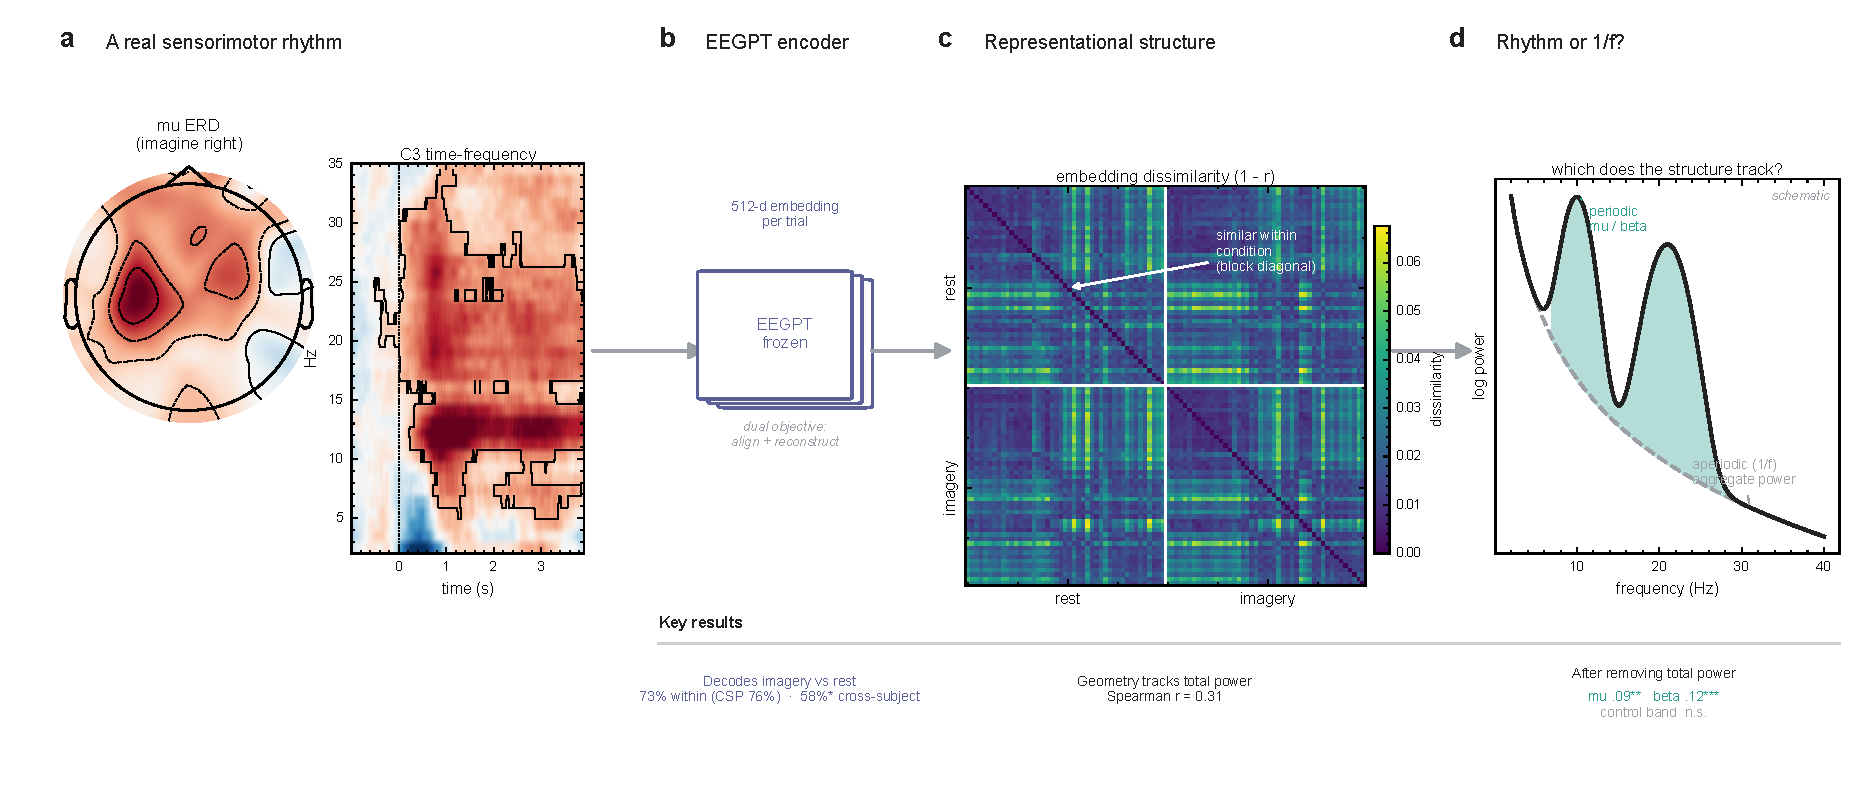
\includegraphics[width=\textwidth]{../figures/fig1_overview.pdf}
\caption{Auditing EEGPT on motor imagery (PhysioNet, $n = 35$ subjects, $2891$
cued $4$~s trials). (a) Grand-average sensorimotor spectrum with its fitted
aperiodic $1/f$ component and the mu peak above it. (b) The embedding geometry
tracks aggregate total power (dashed, $r \approx 0.24$) far more than any
aperiodic-adjusted band; mu sits only ${\approx}0.04$ above the non-motor
controls. (c) Mu and posterior alpha share the $8$--$13$~Hz band, so the trend is
tested against location: alignment is much stronger over central than occipital
electrodes and survives partialling out the other region (dots are subjects).
Electrode regions are channel space, not source localization.}
\label{fig:audit}
\end{figure*}

\section{Discussion}
EEGPT decodes motor imagery competently, yet its representation is organized
primarily by aggregate, largely aperiodic power, with only a small and
consistent trend toward the sensorimotor mu rhythm and no reliable beta trend.
Despite its added alignment objective, the model does not represent the
functional rhythm strongly, which extends the aperiodic and aggregate power bias
reported for reconstruction based models to a hybrid architecture. The balanced
reading for neurotechnology is that EEGPT reliably captures a coarse scale
signal, aggregate and largely aperiodic power, which is itself physiologically
meaningful rather than noise~\cite{donoghue2020specparam}, but it has not yet
shown strong specificity to the finer sensorimotor rhythm; aggregate power is
also the part most perturbed when recording conditions shift across sessions or
devices. Because EEGPT already pairs masked reconstruction with a JEPA-like
latent alignment and still shows only a coarse grounding, the pattern may
reflect current self supervised pretraining broadly rather than any single
objective. The same rhythm versus power lens should therefore be applied to
autoregressive, GPT-style models~\cite{neurogpt2023} and to joint-embedding
predictive (JEPA) models~\cite{assran2023ijepa} alike.

The audit also carries a methodological caution for the interpretability
literature itself: the specificity verdict flipped from non specific to strongly
specific to a small trend as we moved from raw band power to sensorimotor
averaging to a parameterized, spatially controlled analysis. Band power
conflates periodic and aperiodic activity~\cite{donoghue2020bandratio}, and
spatial averaging inflates apparent specificity, so specificity claims about
foundation models should rest on parameterized, spatially controlled measures.

\subsection{Limitations}
The audit covers one model, one dataset, and one paradigm; the RSA is
correlational; the mu trend is small; the spatial control establishes central
weighting in channel space rather than source localization, and because EEG is
volume conducted a central scalp topography constrains but does not identify the
cortical generator; and we have not run a head-to-head against other foundation
models, so we can say the bias persists in EEGPT, not that EEGPT is better or
worse than pure reconstruction models.

\subsection{Future work}
A head-to-head RSA against pure reconstruction models (does the alignment
objective matter), a cross subject RSA asking whether the transferable component
is the rhythm or the power, scaling to more subjects to test whether the mu
trend persists, and a causal attribution or erasure test~\cite{shama2026prism}
would each strengthen the account.

\section{Conclusion}
We audit EEGPT, an alignment plus reconstruction EEG foundation model absent
from prior audits, on motor imagery. It decodes well but represents the task
mainly through aggregate, largely aperiodic power, with only a small, spatially
and spectrally controlled trend toward the sensorimotor mu rhythm. The
specificity verdict depends on the analysis, which is itself a caution for how
these models are audited.

\bibliographystyle{IEEEtran}
\bibliography{refs}

\end{document}
